\documentclass{article}

\usepackage{parskip}
\usepackage{graphicx}

\title{CSCI / MATH 2072U Assignment 2}
\author{Tyson Grant - 100875284}
\date{January 2024}

\begin{document}

\maketitle

\newpage

%'*' used to remove numbering since " 1 Question 1" is not very appealing
\section*{Question 1}
    The purpose of this project is to analyze the different equations in question 1 and use methods from calculus to find a domain enclosing the root of the function that is closest to the origin.  This interval will then be used as an efficient initial domain to start the bisection method to find the root of an equation, minimizing the error, residual, and time taken to solve.  Similar methods have been used for each part of Question 1 with the step process: 
    
    \begin{enumerate}
        \item Plot the graph and observe the domain of the root closest to the origin.
        \item Test the endpoints of this interval in each function $f(x)$, if the signs differ between the values then we know by the Intermediate Value Theorem there exists at least one root in that interval.
        \item Find the Derivative of $f(x)$ and use the sign to determine whether the slope of $f(x)$ is increasing or decreasing.
        \item Analyze the derivative to prove uniqueness over the interval - that there is exactly one root within the interval - using inequalities and previous knowledge of the behaviour of particular functions.  A graph below zero means that the original function will have a negative slope, and vice-versa.
    \end{enumerate}

    
\subsection*{a)}
    \begin{equation}
        [ f(x) = (x-1)\cos(x)+\frac{1}{2}
    \end{equation}

    To start, we must plot Equation 1 and analyze the graph to find a good initial domain to be chosen for Bisection.  The initial domain of (a,b) was chosen to be (0,1). To prove there is a root within this domain (a,b) we must test the endpoints in Equation 1 and verify the y-values change signs, proving that there is a root:

    \begin{equation}
         f(a) = f(0) = (0-1)\cos(0)+\frac{1}{2} = -\frac{1}{2} 
    \end{equation}
    \begin{equation}
         f(b) = f(1) = (1-1)\cos(1)+\frac{1}{2} = \frac{1}{2} 
    \end{equation}
    
    Therefore, $f(a) < 0$ and $f(b) > 0$, so $f(a)f(b) < 0$, the function must cross the x-axis over the interval, so by the Intermediate Value Theorem (IVT) there is at least one root exists between (0,1).

    Next, we have to prove uniqueness in the interval (a,b).  This can be done by finding the derivative of Equation 1, $f'(x)$ or $\frac{df}{dx}$, and using knowledge of Calculus combined with inequalities, show that Equation 1 is strictly increasing or decreasing which proves there can only be one root within the interval (a,b).
   \begin{equation}
            f'(x) = \cos(x) - (x-1)\sin(x) 
   \end{equation}

    Now we can split up Equation 4 and analyze each part individually within the interval (0,1).  We know that $\cos(x)$ has a period of 2$\pi$, start at (0,1) and intersecting the x-axis at $(\frac{\pi}{2},0)$ and $(\frac{3\pi}{2}$.  Similarly, $\sin(x)$ also has a period of $2\pi$, with roots of $(\pi, 0)$ and $(2\pi,0)$. From this we know $\cos(x) > 0$ and $\sin(x) \ge 0$ within the interval (0,1).  Similarly, we know $(x-1) \le 0$ since it is a constant slope starting at the origin, which implies that $-(x-1) \ge 0$.  Using these inequalities, we can conclude that $f'(x) > 0$.  Which states that the derivative is always positive, proving Equation 1 is always above the x-axis.  These facts lead to the conclusion that there is precisely one root in the interval (0,1).  Therefore to use the Bisection method to find convergence, an efficient initial domain 

\subsection*{b)}
    \begin{equation}
             f(x) = \sqrt{x^2+1} -x^3
    \end{equation}

    We need to plot Equation 5 and observe the graph the graph to find an accurate initial domain (a,b).  The initial domain found by plotting the graph was (1,2).  To prove there is a root within the domain, we must test the values of each endpoint in Equation 5 to check if it intersects the x-axis.

    \begin{equation}
             f(a) = f(1) = \sqrt{2^2+1} -2^3 = 0.414
    \end{equation}
    \begin{equation}
        f(b) = f(2) = \sqrt{2^2+1} -2^3 = -5.55
    \end{equation}

    Therefore, $f(a) > 0$ and $f(b) < 0$, so $f(a)f(b) < 0$, so by the IVT we can conclude that there exists at least one root within the interval (1,2) for the Equation 5.

    Next, we have to prove there is exactly one root within the interval.  We must calculate the derivative of Equation 5, $f'(x)$, and show it is strictly increasing or decreasing throughout the interval.
    \begin{equation}
         f'(x) = \frac{x}{\sqrt{x^2+1}}-3x^2 
    \end{equation}

    Now, we can break up the derivative and use inequalities to prove the function is always increasing or decreasing in the interval (1,2).    
    
    For all $x \in {\rm I\!R}|x>0$, $\frac{1}{\sqrt{x^2+1}} < -3x^2$, ($x > 0$ taken as argument since a downward-facing parabola with no translations has maximum at origin).  Since $3x^2$ is being subtracted from $\frac{x}{\sqrt{x^2+1}}$ (always smaller than $3x^2$), and $\frac{x}{\sqrt{x^2+1}}$ can never be greater than 1, we can imply that Equation 8 will always equate to a negative value. 
    
    Using these inequalities, it is evident that Equation 8 is always below the x-axis (less than zero) within the interval (1,2).  This proves that the slope of Equation 5, $f(x)$, is always decreasing through the interval of (1,2), so there can only exist precisely one root.  Therefore, an efficient initial domain to use in the Bisection iteration method for Equation 5 would be (1,2).

\subsection*{c)}
    \begin{equation}
        f(x) = x\ln(x)-2x+x^2+1
    \end{equation}

    When observing the graph of Equation 9, it can be seen that a good initial domain (a,b) to choose would be (0.1,0.5).  This interval was chosen to a precise degree due to the condensed x-axis of the graph, with there is two intercepts before $x=1$.  Also, using $a=0$ does not work with this function because Equation 9 is undefined at x=0, since $\ln(0) = undefined$. Next, we need to prove there is a root within the chosen interval.

    \begin{equation}
         f(a) = f(0.1) = 0.1\ln(0.1)-2(0.1)+(0.1)^2+1 = 0.579 
    \end{equation}
    \begin{equation}
         f(b) = f(0.5) = 0.5\ln(0.5)-2(0.5)+(0.5)^2+1 = -0.097 
    \end{equation}

    Therefore, $f(a) > 0$ and $f(b) < 0$ so $f(a)f(b) < 0$, proving by IVT that there is at least one root in the set interval of the function $f(x)$.  

     Next, we have to prove uniqueness within the interval (0.1, 0.5).  We must calculate the derivative $f'(x)$, then show it is either always increasing or decreasing.
     \begin{equation}
         f'(x) = \ln(x)+2x-1
     \end{equation}

    Now we can break up Equation 12 into sections and analyze each piece to determine if function is increasing or decreasing over the interval (0.1,0.5).  We know $ln(x)$ is always increasing and intersects the x-axis at $x=1$ so it is positive over the interval, and is undefined at $x=0$.  On the interval (0.1,0.5): $\ln(x) < 0$, and $2x-1 \le 0$ since the y-intercept would be $y=-1$ with $\frac{rise}{run} = \frac{2}{1}$.  Therefore, using these inequalities we can say that $f'(x) < 0$ over the interval (0.1,0.5).  This proves that Equation 9 will always have a decreasing slope over the interval (0.1,0.5).  In conclusion, there can only exist a single root over the interval (0.1,0.5) for Equation 9, the decreasing slope does not allow the function to 'turn around'.

\subsection*{d)}
    \begin{equation}
         f(x) = \frac{1}{(x+1)^2} + \frac{4}{(x+2)^2} -1
    \end{equation}

    When observing the graph of Equation 13, it is evident that an efficient initial domain (a,b) to start bisection would be (0,1).  This is proven by using the following.  First, we have to prove there is a root within the selected domain.  In order to do this we must calculate $f(a)$ and $f(b)$ for our endpoints, and check if the signs flip between the two which would prove there is an intersection of the x-axis within the interval.

    \begin{equation}
         f(a) = f(0) = \frac{1}{(0+1)^2} + \frac{4}{(0+2)^2} -1 = 1
    \end{equation}
    \begin{equation}
         f(b) = f(1) = \frac{1}{(1+1)^2} + \frac{4}{(1+2)^2} -1 = -0.306
    \end{equation}

    Consequently, $f(a) > 0$ and $f(b) < 0$, so $f(a)f(b) < 0$, so by the IVT we can state that there exists at least one root within the interval (0,1).
    
    Then, we must prove that there is exactly one root within the interval.  To do this we must calculate the derivative of Equation 13,$f'(x)$, and use inequalities to show that it is either increasing or decreasing through the entire interval.

    \begin{equation}
        f'(x) = -\frac{2}{(x+1)^3} - \frac{8}{(x+2)^3} 
    \end{equation}

    Similar to the other questions, we break up the derivative into sections and use inequalities to determine if each section is positive or negative.  From mathematical and graphical knowledge, we know that the denominators of Equation 13 cause vertical asymptotes at $y=-2$ and $y=-1$.  We also know that $\frac{1}{(x+1)^3} > 0$ when $x>-1$ due to vertical asymptote, so $-\frac{1}{(x+1)^3} < 0$ when $x>1$, so $-\frac{2}{(x+1)^3} < 0$ when $x>-1$.  Similarly, $\frac{1}{(x+2)^3} > 0$ when $x>-2$ due to vertical asymptote, so $-\frac{1}{(x+2)^3} < 0$ when $x>-2$, then $-\frac{8}{(x+2)^3} < 0$ when $x>-2$.  Since the values of each derivative are always less than zero, and the two are subtracted, we have shown that $f'(x) < 0$ for all values within the interval, so the function $f(x)$ has a decreasing (negative) slope through the interval (0,1).  In conclusion, there can only exist exactly one root over the interval of (0,1) for the function $ f(x)$.

\subsection*{e)}
    \begin{equation}
         f(x) = e^{-x^3+x-2}-\frac{1}{10}
    \end{equation}

    After plotting the Equation 17 on a graph, it can be seen that a efficient initial domain would be (-0.5,0).  Due to the nature of the exponential function we know there is a horizontal asymptote at $y=0$, but in this case the translation of $-\frac{1}{10}$ the asymptote has been phase shifted down to $y=-\frac{1}{10}$.  Next, we have to prove that the IVT holds true over the interval (-0.5,0), which can be done by calculating the endpoint, $f(a)$ and $f(b)$, in Equation 17 for our domain (-0.5 0).

    \begin{equation}
         f(a) = f(-0.5) = e^{-(-0.5)^3+(-0.5)-2}-\frac{1}{10} = -0.007 
    \end{equation}
    \begin{equation}
         f(b) = f(0) = e^{(-0^3+0-2)}-\frac{1}{10} = 0.035
    \end{equation}

    Since $f(a) < 0$ and $f(b) > 0$, then $f(a)f(b)$, so we can say that the IVT holds true proving that there is at least one root that exists over the interval (-0.5,0).

    The next step taken is to calculate the derivative to prove that the function has a slope that is either always increasing or decreasing within the interval, to draw the conclusion that there exists a unique root over the interval.

    \begin{equation}
         f'(x) = e^{-x^3+x-2}(-3x^2+1) 
    \end{equation}

    Using the calculation of the derivative and inequalities, we can prove the $f'(x)$ is positive or negative which would result in a respective increasing or decreasing slope of $f(x)$.  Utilizing properties of a quadratic, we know that $x^2 >= 0$ with a minimum of (0,0), so $-x^2 \le 0$ with maximum at (0,0), then $-3x^2 \le 0 $, but the vertical translation of '+1' causes $(-3x^2+1)$ to now have a maximum at (0,1).  Solving a quadratic gives the roots of $\pm\frac{1}{\sqrt{3}}$, and due to the maximum being at (0,1) it is evident that $(-3x^2+1) > 0$ for the interval (-0.5,0).  We also know that $e^x$ has a horizontal asymptote at $y=0$, so $e^z)$ is positive for any value of z (including functions). To recap, on the interval (-0.5,0): $(-3x^2+1) > 0$, and $e^{-x^3+x-2} > 0$.  Therefore by the use of the inequalities, we have shown that derivative $f'(x)$ is always positive over the interval (-0.5,0).  This proves that the function $f(x)$ has a positive slope throughout the entire interval selected.  To conclude, there can only exist exactly one root over the interval (0.1,0.5) for the given function.

\newpage
\section*{Question 2}

    %PDF COULD NOT BE SAVED IF INSERTED FIGURES IN LATEX FILE, SO HAD TO EDIT IT AFTER DOWNLOADING AND INSERT PLOTS

    \begin{figure}[!htb]
        \centering
        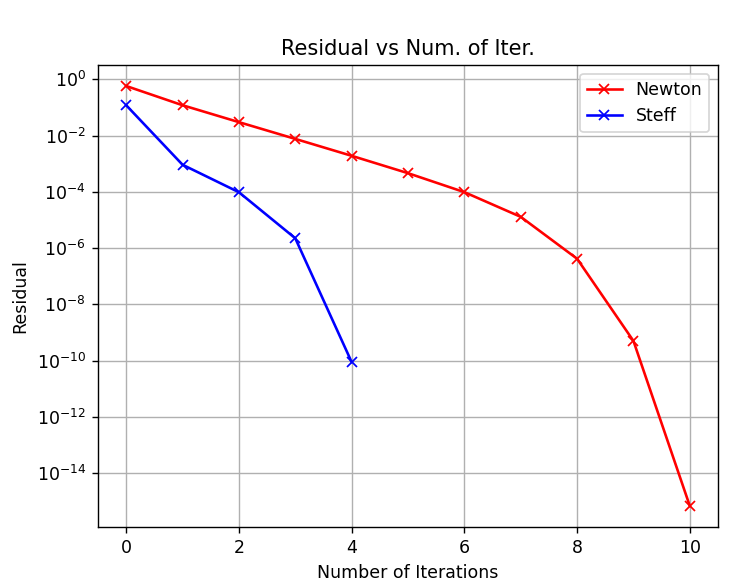
\includegraphics[width=0.5\linewidth]{res_plot.png}
        \caption{Analyzes Residual decrease with each iteration}
        \label{fig:1}
    \end{figure}

    \begin{figure}[!htb]
        \centering
        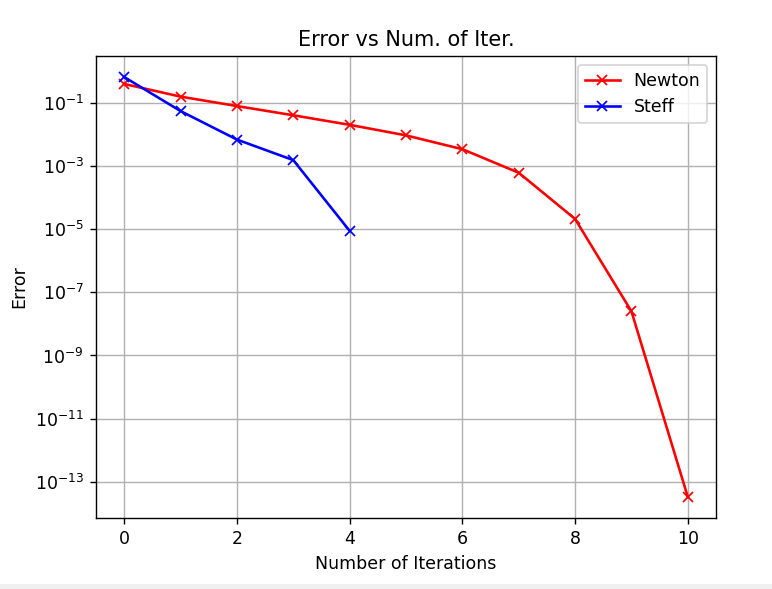
\includegraphics[width=0.5\linewidth]{err_plot.png}
        \caption{Analyzes Error decrease with each iteration}
        \label{fig:2}
    \end{figure}

        As can be seen from the Figure 1 and Figure 2, the Newton iteration method does not have a quadratic convergence, unlike the Steffensen method.  The Newton method starts off with a linear increase but then begins to exponentially increase, whereas Steffensen's method has a relatively quadratic behaviour as it increases.

        Using these Figures, it is evident that the Steffensen iteration is more efficient since it took 5 iterations to converge whereas Newton iteration took 11 iterations to reach the convergence point.  This will remain true for all functions, Steffensen has proven to be more efficient.
        
\end{document}
